\section{Interval Scheduling as Graph Problems}

There is a natural way to view the interval scheduling and partitioning problems as graph problems.

\index{intersection graph} \index{interval graph}
Let $I$ be a set of intervals. We can construct the \textbf{intersection graph} $G(I) = (V,E)$ where $V=I$ and $(u,v) \in E$ if and only if the intervals corresponding to $u$ and $v$ intersect.

Any graph that is the intersection graph of a set of intervals is called an \textbf{interval graph}. The interval scheduling and interval partition problem can be viewed as the \textbf{maximum independent set problem} for the class of interval graphs.

\begin{definition}[Maximum Independent Set]
    Let $G=(V,E)$ be a graph. A subset $U$ of $V$ is an independent set (stable set) in $G$ if for all $u,v \in U$, $(u,v) \not\in E$.

    The maximum independent set of $G$ is an independent set of $G$ with maximum cardinality.
\end{definition}

\begin{pitfall}
    Maximal and maximum are \textit{\textbf{not}} the same. It is important to distinguish between ``maximum'' and ``maximal'' sets, and between ``minimum'' and ``minimal'' sets. A maximal set is a set that is not a proper subset of any other sets, while a maximum set is simply a set of maximum cardinality among all sets.
\end{pitfall}

\begin{figure}[htbp]
    \centering
    \includegraphics[width=0.6\linewidth]{greedy/Interval_graph.pdf}
    \caption{Intervals represented as an interval graph. Image from \href{https://en.wikipedia.org/wiki/Interval_graph}{Wikipedia}.}
    \label{fig:greedy-interval-graph}
\end{figure}

\begin{definition}[Graph Coloring]
    Let $G=(V,E)$ be a graph. A function $c:\, V \to \{1,\ldots,k\}$ is a valid coloring of $G$ if $c(u) \neq c(v)$ for all $(u,v) \in E$.

    The graph coloring problem is to find a coloring $c$ that minimizes the number of colors $k$. Such number is called the chromatic number of $G$, denoted $\chi(G)$.
\end{definition}

To model the interval scheduling and partition problem as a graph theory problem, we first need a way to efficiently interconvert between the interval graph representation and the set representation.

Given a set $I$ of intervals, it is easy to construct the interval graph $G(I)$. For conversion back from interval graph, the following theorem claims that it can also be done efficiently.

\begin{theorem}
    Given any graph $G$, there is a linear-time algorithm to decide if $G$ is an interval graph, and if so, to construct an interval representation.
\end{theorem}

The maximum independent set problem for intersection graph can be efficiently solved, so the interval scheduling and partition problem can also be efficiently solved. The graph theoretical explanation for this is that interval graphs are chordal graphs with a perfect elimination ordering, making it possible to use the greedy approach (or more generally, a priority based approach). However, in the general case, the maximum independent set problem is known to be NP-hard.

To formallly prove that the maximum independent set problem can be efficiently solved for interval graphs, we need to introduce a few additional concepts.

\subsection{Interval Graph is Chordal Graph}

We first show that an interval graph is also a chordal graph (the converse is not true).

\begin{definition}[Chordal Graph] \index{chordal graph} \index{rigid circuit graph} \index{chord}
    Let $G$ be an undirected graph. $G$ is a \textbf{chordal graph} or \textbf{rigid circuit graph} if for any cycles of 4 or more vertices, there exists a pair of vertices $u,v$ on the cycle such that $\{u,v\} \in E$. The edge $\{u,v\}$ is called a \textbf{chord} of the cycle.
\end{definition}

\vspace{\parskip}

\begin{theorem}
    An interval graph is also a chordal graph.
\end{theorem}

\begin{proof}
    Let $G=(V,E)$ be an interval graph with a cycle $C_k = v_1v_2\ldots v_kv_1$ where $k \geq 4$ and each $v_i$ represents an interval $[a_i,b_i)$. The case where $k < 4$ is vacuously true. Suppose the first $k$ vertices of the cycle are ordered in increasing order by the left endpoints of the intervals they represent. Consider the $k$ vertex on the cycle. $\{v_{k-1},v_k\} \in E$, so $[a_{k-1},b_{k-1}) \cap [a_k,b_k) \neq \emptyset$. Since the vertices are sorted by left endpoints, $a_k \in [a_{k-1},b_{k-1})$. Since $C_k$ is a cycle, $\{v_k,v_1\} \in E$, so $[a_1,b_1) \cap [a_k,b_k) \neq \emptyset$. Again, because the intervals are sorted by left endpoints, $a_1 < a_k$. It follows that $a_k \in [a_1,b_1)$. $a_k$ is in both the interval $[a_{k-1},b_{k-1})$ and $[a_1,b_1)$, so $[a_1,b_1) \cap [a_{k-1},b_{k-1}) \neq \emptyset$, so $\{v_1,v_{k-1}\} \in E$ by definition of interval graphs. $\{v_1,v_{k-1}\}$ is a chord, so $G$ is a chordal graph.
\end{proof}

\subsection{Perfect Elimination Ordering and Cliques}

The next step is to show that there exists an ordering of the vertices of the interval graph, from which we can derive a greedy algorithm.

\begin{definition}[Simplicial Vertex]
    In a graph $G=(V,E)$, we say $v \in V$ is \textbf{simplicial} if the subgraph induced by the $\{v\} \cup N(v)$ is a complete graph (forms a clique).
\end{definition}

\begin{definition}[Perfect Elimination Ordering]
    A graph $G=(V,E)$ has a \textbf{perfect elimination ordering (P.E.O.)} if there is an ordering $(v_1,\ldots,v_n)$ of $V$ such that $v_i$ is simplicial vertex in the subgraph induced by $\{v_i,\ldots,v_n\}$. 
\end{definition}

\begin{definition}[Separator and Minimal Separator]
    Given a graph $G=(V,E)$, we define the \textbf{separator} $S$ in $G$ to be the subset of $V$ such that it partitions $V$ into three disjoint sets $A,S,B$ such that $V=A\cup S \cup B$ and for all $a \in A$ and $b \in B$, $(a,b) \not\in E$. Intuitively, this means there is no edge going directly from a vertex in $A$ to a vertex in $B$, so the subgraph induced by $V-S$ has two disjoint connected components (induced by $A$ and $B$).

    Given two non-adjcent vertices $a,b \in V$ such that $(a,b) \not\in E$, we say $S$ is an $\mathbf{(a,b)}$-\textbf{separator} if $S$ partitions $V$ into disjoint subsets $A,S,B$ such that $a \in A$ and $b \in B$. A \textbf{minimal} $(a,b)$-separator is an $(a,b)$-separator $S$ such that no subset of $S$ is an $(a,b)$-separator.
\end{definition}

\begin{figure}[htbp]
    \centering
    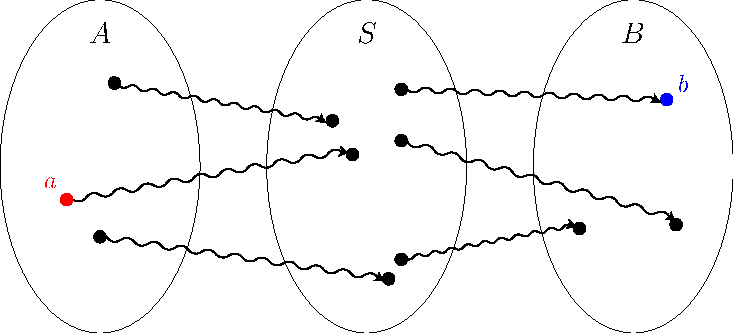
\includegraphics[width=0.5\linewidth]{greedy/graph-ab-separator.pdf}
    \caption{Example of an $(a,b)$-separator}
    \label{fig:graph-ab-separator}
\end{figure}

\begin{lemma} \label{lem:chordal-implies-separation}
    Given a chordal graph $G=(V,E)$ and two non-adjacent vertices $a,b \in V$ such that $(a,b) \not\in V$, any minimal $(a,b)$-separator induces a clique.
\end{lemma}

\begin{proof}
    By contradiction.

    Let $S$ be a minimal $(a,b)$-separator. Let $A,B$ be the two connected components separated by $S$, where $a \in A$ and $b \in B$. Suppose, for contradiction, that $S$ does not induce a clique, so there exists $u,v \in S$ such that $\{u,v\} \not\in E$. Since $S$ is minimal, there are edges from $u$ and $v$ to the subgraphs induced by $A$ and $B$. Otherwise, $S-\{u,v\}$ would have been a smaller $(a,b)$-separator.

    Let $p_a$ be the shortest path from $u$ to $v$, passing through vertices in $A$. Similarly, let $p_b$ be the shortest path from $v$ to $u$, passing through vertices in $B$. $p_a$ and $p_b$ each has path length of at least 2 because $u,v$ are not adjacent. It follows that the union of the two paths $p_a$ and $p_b$ is a cycle $u \to a_1 \leadsto a_k \to v \to b_1 \leadsto b_k \to u$ of length at least 4. Since $G$ is chordal, this cycle must contain a chord. But since this is the shortest cycle, there is no edge from $u,v$ to vertices in $A,B$ (otherwise, we can form a shorter cycle using this edge). There is no edge from vertices in $A$ to vertices in $B$ because the subgraphs they induce are disjoint. So, the chord must be between $u$ and $v$. However, this contradicts the assumption that $\{u,v\}\not\in E$.

    Hence, for every $u,v \in E$, $\{u,v\} \in E$.

    \begin{center}
        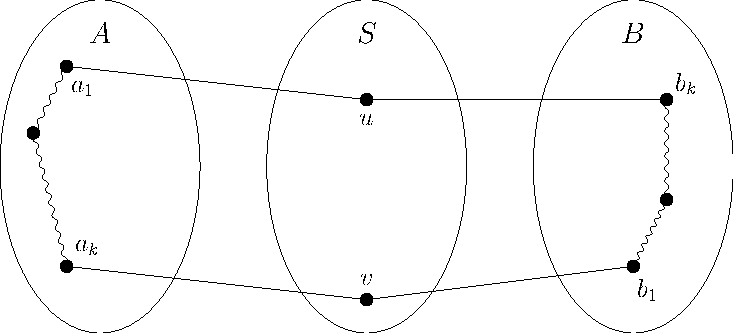
\includegraphics[width=0.5\linewidth]{greedy/graph-ab-sep-shortest-cycle.pdf}
    \end{center}
\end{proof}

\begin{lemma}[Dirac 1961] \label{lem:separation-implies-peo}
    Given a graph $G=(V,E)$, if all for all $a,b\in V$, the minimal $(a,b)$-separator induces a clique, then $G$ has a perfect elimination ordering.
\end{lemma}

\begin{proof}
    By induction on the number of vertices in $G$.

    \textbf{Base case}: When $n=1$, the lemma trivially holds.

    \textbf{Inductive step}: Let $n \in \N$. Assume that the lemma holds for all $k < n$.

    If $G$ is a complete graph, the whole graph is a clique, and we are done since every ordering is a perfect elimination ordering.

    Otherwise, there exists $a,b \in V$ such that $\{a,b\} \not\in E$. Let $S$ be a minimal $(a,b)$-separator in $G$. $S$ separates $V$ into disjoint subsets $A,S,B$. By assumption, $S$ induces a clique. Since the size of $A$ is strictly smaller than $V$, by induction hypothesis, we know that $A$ has a perfect elimination ordering. This implies that there exists $u \in A$ such that $\{u\} \cup N(u)$ induces a clique on the subgraph induced by $A$.

    Since $S$ separates $A$ and $B$, there is no edge going directly from vertices in $A$ to vertices in $B$. There is an edge connecting every pair of vertices in $S$, so if there are edges going between $u$ to vertices in $S$, the resulting subgraph is also a clique. Hence, $\{u\} \cup N(u)$ also induces a clique in $G$ because $S$ induces a clique.

    Consider the graph $G'$ obtained by removing vertex $u$ from $G$. $|V-\{u\}| < |V| = n$. By induction hypothesis, $G'$ has a perfect elimination ordering. Suppose the ordering is $(v_1,\ldots,v_{n-1})$. We can let $v_n = u$. By adding $v_n$ to the ordering, we get a new valid perfect elimination ordering because $v_{n}$ and its neighbors induces a clique in $G$.
    
    By induction, the lemma holds for graph of any size.
\end{proof}

\begin{figure}[htbp]
    \centering
    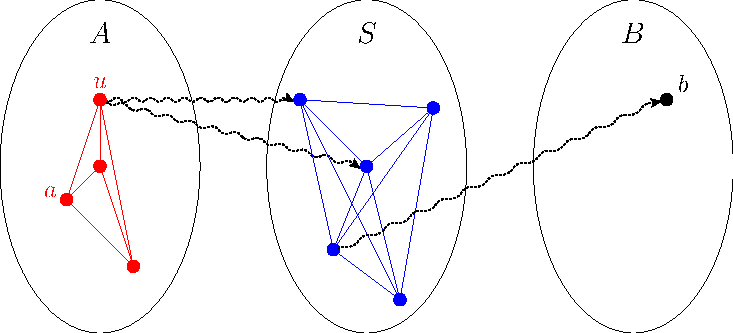
\includegraphics[width=0.5\linewidth]{greedy/graph-clique-separation.pdf}
    \caption{Proof idea for Lemma \ref{lem:separation-implies-peo}}
    \label{fig:graph-clique-separation}
\end{figure}

\begin{theorem}[Fulkerson and Gross 1965]
    A graph is a chordal graph if and only if it has a perfect elimination order.
\end{theorem}

\begin{proof}
    We will prove the theorem by proving the chain of implications that
    $$
    \text{(1) P.E.O.} \Rightarrow \text{(2) chordal graph}\Rightarrow \text{(3) minimal separator induces a clique} \Rightarrow \text{(1) P.E.O.}
    $$
    (1) $\Rightarrow$ (2): Let $C$ be a cycle of length at least 4 in $G$. Assume $G$ has a perfect elimination ordering. Then, take the perfect elimination ordering, and remove vertices by the ordering until we reach a vertex $c$ on the cycle $C$. Once we remove $c$, $N(c)$ induces a clique by definition of perfect elimination ordering. Therefore, there exists an edge between every two vertices in $C-\{c\}$. In other words, $C$ contains chords. Hence, $G$ is a chordal graph.

    (2) $\Rightarrow$ (3): By Lemma \ref{lem:chordal-implies-separation}.

    (3) $\Rightarrow$ (1): By Lemma \ref{lem:separation-implies-peo}.
\end{proof}

Tarjan and Yannakakis designed a linear-time algorithm called the maximum cardinality search for computing the perfect elimination ordering given a chordal graph \cite{Tarjan-Chordal-Graph}.

\begin{codebox}
    \Procname{$\proc{Compute-PEO}(G)$}
    \li \For all $v \in V$ \Do
        \li $\attrib{v}{label} = 0$
        \li $\sigma(v) = -1$ 
    \End
    \li \For $i=|V|$ \Downto 1 \Do
        \li $u = \mathrm{argmax}_{v \in V} \{ \attrib{v}{label} \mid \sigma(v) = -1 \}$ \quad \Comment{unvisited vertex with largest label}
        \li $\sigma(u) = i$ \quad \Comment{assign an order}
        \li \For neighbor $w$ of $v$ \Do
            \li \If $\sigma(w) \isequal -1$ \Then
                \li $\attrib{w}{label} = \attrib{w}{label} + 1$
            \End
        \End
    \End
    \li \Return $\sigma$
\end{codebox}

The algorithm starts by initializing the labels and numbers for each vertex. Then, it iteratively select unnumbered vertex with largest label to assign an order. With an naive implementation, Line 5 of the algorithm takes $O(|V|)$ time. However, this can be improved by using a disjoint set data structure. Let $S_i$ be the sets of unnumbered vertices with label $i$ for $0 \leq i \leq |E|-1$. Each $S_j$ is implemented using a linked list, and $[S_0,S_1,\ldots S_{i} ]$ is a direct access array indexed by $i$. Every time we increment the label of $w$, we move $w$ from $S_{i}$ to $S_{i+1}$ where in this case, $i$ is the $\attrib{w}{label}$. It is clear that this improved implementation runs in $O(|V|+|E|)$ time.

Finally, as promised, we will show an algorithm that solves the maximum independent set problem on an interval (chordal) graph.

\begin{codebox}
    \Procname{$\proc{MIS}(G)$}
    \li $\sigma = \proc{Compute-PEO}(G)$
    \li $I = \emptyset$
    \li \For $i = 1$ \To $|V|$ \Do
        \li $v = \sigma^{-1}(i)$
        \li $N = \{v \in N(v) \mid \sigma^{-1}(v) < i \}$
        \li \If $N \cap I \isequal \emptyset$ \Then
            \li $I = I \cup \{v\}$
        \End
    \End
    \li \Return $I$
\end{codebox}

The proofs in this section are based on the papers \textit{Incidence matrices and interval graphs} by Fulkerson and Gross \cite{Fulkerson1965-Chordal-Graph}, and \textit{On rigid circuit graphs} by Dirac \cite{Dirac1961-Rigid-Circuit-Graph}. The presentation of the proofs is loosely based on \textit{Advanced Topics in Graph Algorithms} by Ron Shamir \cite{shamir}.

\section{Minimum Spanning Tree}

\subsection{Kruskal's Algorithm}

\subsection{Prim's Algorithm}

\section{Single-Source Shortest Path}

\subsection{Dijkstra's Algorithm}